\documentclass[11pt]{article}

\usepackage{preamble}
\usepackage{tocloft}
\setcounter{tocdepth}{1}
\renewcommand{\cftsecleader}{\cftdotfill{\cftdotsep}}

\begin{document}
    \begin{titlepage}
        \center
        % University
        \textsc{\LARGE University of Moratuwa}\\[.5cm]

        % Document info
        \textsc{\Large Circuits And System Design}\\[0.2cm]
        \textsc{\large EN3030}\\[1cm]                                        % Course Code
        \HRule \\[0.4cm]
        { \Large \bfseries ASSIGNMENT : WEEK 01}\\[0.25cm]
        \HRule \\[1cm]
        \large
        \textbf{\emph{\large Team : INFOS}}\\
        [0.3cm]
        \begin{tabular}{ |l| c|c| }
            \toprule
            Yasarathna D.D.K.B. & 190719V & Ex - 01 \\
            \midrule
            Tharindu.O.K.D      & 190622R & Ex - 02 \\
            \midrule
            S.Sanjith           & 190562G & Ex - 03 \\
            \midrule
            K.Kajhanan          & 190286M & Ex - 04 \\
            \midrule
        \end{tabular}\\
        [.5cm]
        {\large \today}\\[1cm]
        
\includegraphics[width=0.4\textwidth]{mora.png}\\[1cm]    % University logo
        \tableofcontents
        \vfill
        \HRule
        \flushleft {Executable codes can be found \href{https://github.com/University-Academics/INFOS}{here}}
    \end{titlepage}


    \section{Floating Point Addition/Subtraction}

    \subsection{IEEE-754 Single Precision Format}
    \begin{figure}[h]
        \begin{center}
            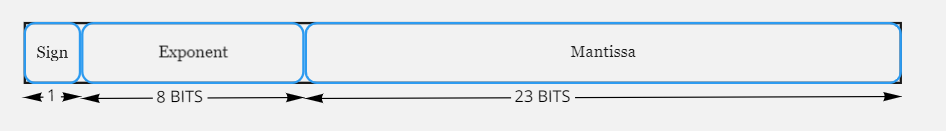
\includegraphics[width=.7\textwidth]{ieee}
        \end{center}
    \end{figure}
    For the verification purposes \href{https://www.h-schmidt.net/FloatConverter/IEEE754.html}{h-schmidt}, an online floatconverter is used.

    \subsection{Algorithm}
    \begin{enumerate}
        \item Compare the exponents of two numbers and find the absolute difference.
        \item Shift the number with the smaller exponent to right by the amount of absolute difference to make the exponents of both numbers equal. Assign the prominent exponent as the exponent of the sum.
        \item Check the signs of two numbers after performing sign conversion according to operation
        \begin{itemize}
            \item If both are of the same sign add two corresponding mantissa and assign it to sum\_mantissa.
            \item Otherwise, subtract the matissa of number with 1 as sign bit from the other and assign the magnitude of it as sum\_mantissa.
        \end{itemize}
        %\hspace*{\dimexpr\linewidth-\textwidth\relax} At this stage, sum mantissa will contain 25bits to accomadate the overflow.
        \item Assign the sum\_sign according to sign of two numbers and above derived answer.
        \item Shift the mantissa left until and 24th-bit position of the mantissa is one and reduce the exponent of the sum accordingly(normalization)
        \item Now discard the implicit 1 and consider only the lower 23-bits of sum\_mantissa.
        \item Final Answer = \{sum\_sign, sum\_exponent, sum\_mantissa\}
    \end{enumerate}
    Visual implementation of the given algorithm as a flowchart is attached to this report in the end.

    \subsection{Results}
    The following results obtained from illustrated conditions ensure proper functioning of the unit.
    \begin{figure}[h]
        \begin{minipage}{.45\textwidth}
            \begin{center}
                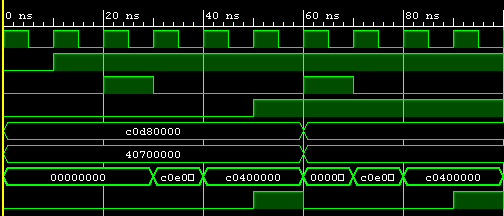
\includegraphics[width=.95\columnwidth]{operation-6.75_3.75}
                \caption*{-6.75+3.75 = -3 \& -6.75-(-3.75) = -3}
            \end{center}
        \end{minipage}
        \begin{minipage}{.45\textwidth}
            \begin{center}
                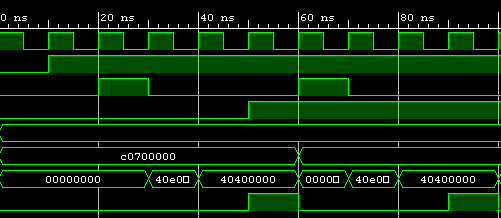
\includegraphics[width=.95\columnwidth]{6.75-3.75}
                \caption*{6.75-3.75 = 3 \& 6.75+(-3.75) = 3}
            \end{center}
        \end{minipage}
    \end{figure}
    \newline
    \begin{tabular}{l l}
        ROW 1 : & Clock \\
        ROW 3 : & Validity of Answer\\
        ROW 5 : & Number 1 \\
        ROW 6 : & Number 2 \\
        ROW 7 : & Sum
    \end{tabular}
    \vspace{.2cm}
    \newline
    Addition and Subtraction indicated above are choosen in a way to return the same result. During the true value of valid entry simulation returns same result for each operation.

\newpage
\appendix
    \section{FP Add/Sub Implementation}
    \begin{figure}[h]
        \begin{center}
            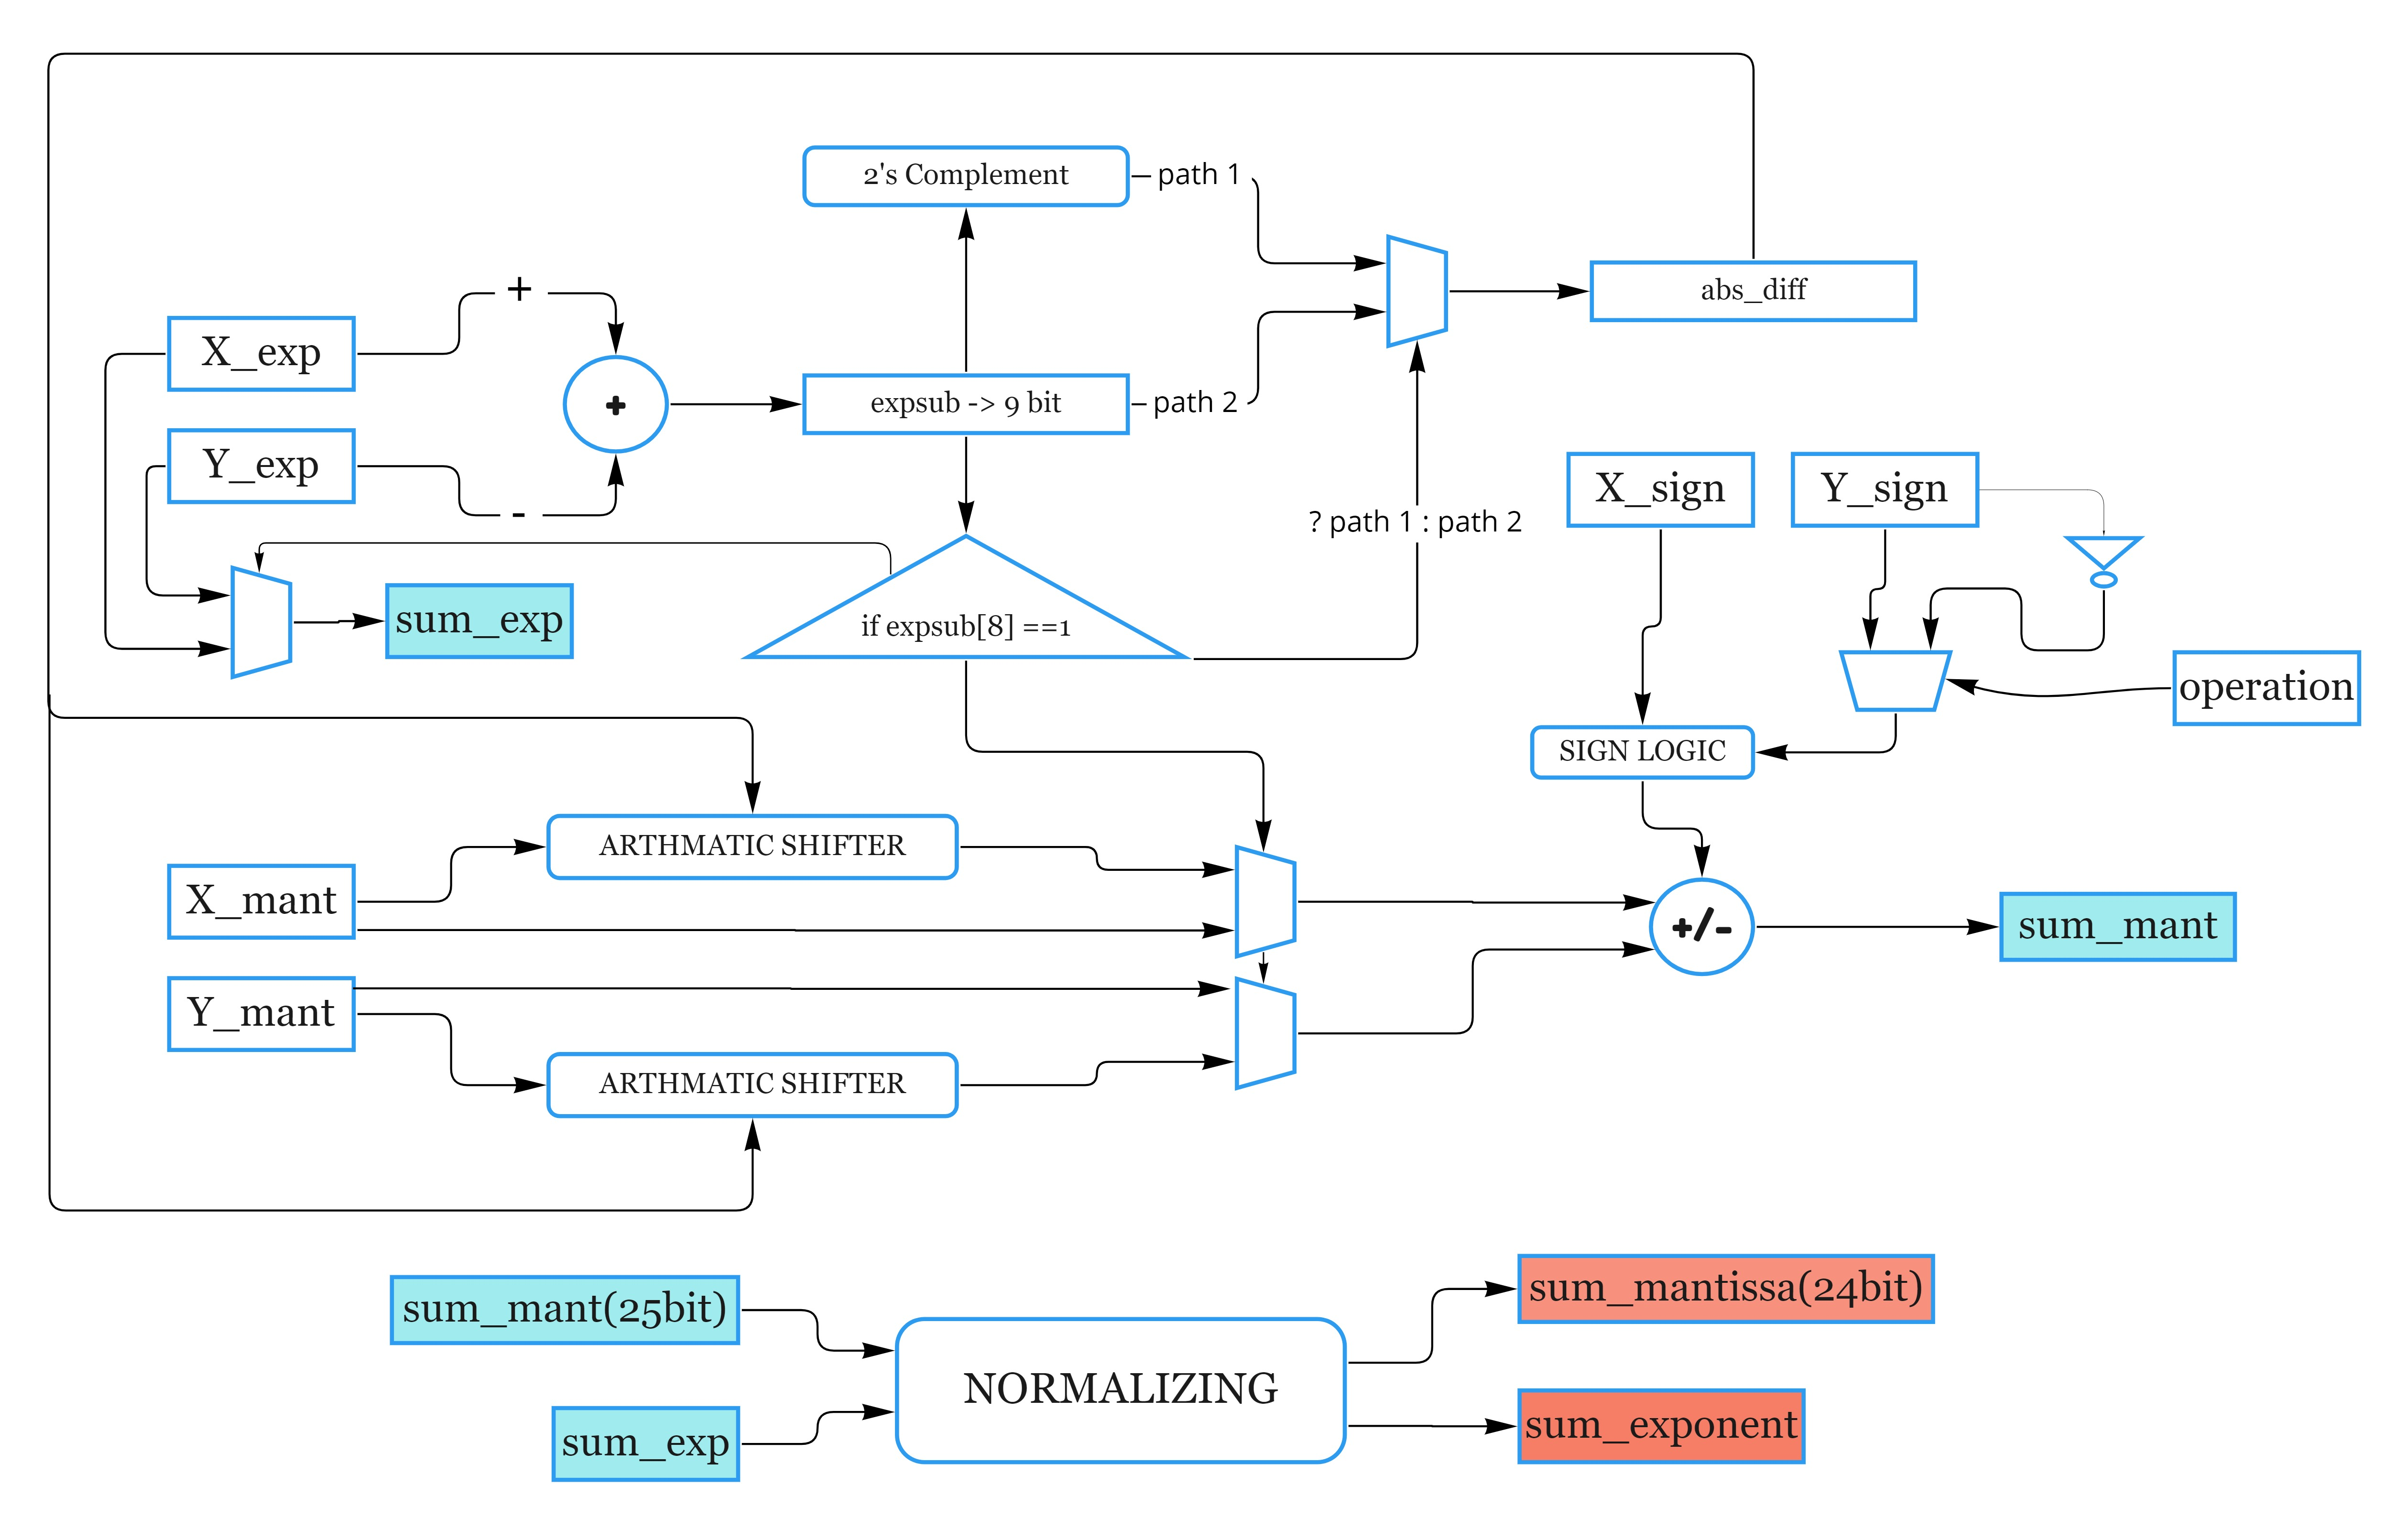
\includegraphics[width=\textwidth]{algorithm}
        \end{center}
    \end{figure}
\end{document}
